\documentclass[letterpaper, 10 pt, conference]{ieeeconf}  % Comment this line out if you need a4paper

%\documentclass[a4paper, 10pt, conference]{ieeeconf}      % Use this line for a4 paper

\IEEEoverridecommandlockouts                              % This command is only needed if 
                                                          % you want to use the \thanks command

\overrideIEEEmargins                                      % Needed to meet printer requirements.

% The following packages can be found on http:\\www.ctan.org
\usepackage{graphics} % for pdf, bitmapped graphics files
%\usepackage{graphicx}
\usepackage[dvipdfmx]{graphicx}
\usepackage[dvipdfmx]{color}
\usepackage{epsfig} % for postscript graphics files
\usepackage{mathptmx} % assumes new font selection scheme installed
\usepackage{times} % assumes new font selection scheme installed
\usepackage{amsmath} % assumes amsmath package installed
\usepackage{amssymb}  % assumes amsmath package installed
\usepackage{multicol}
\usepackage{multirow}
\usepackage{url}
\usepackage{caption}
\usepackage[ruled,vlined]{algorithm2e}
%\include{pythonlisting}
\usepackage{algpseudocode}
\usepackage[dvipsnames]{xcolor}
\usepackage{cite}

\setlength\textfloatsep{5pt}

\title{\LARGE \bf
Time-Based Current Source (TBCS): A Highly Digital Robust Current Generator for Switched Capacitor Circuits
}

\author{Kentaro Yoshioka% <-this % stops a space
%\thanks{*This work was not supported by any organization}% <-this % stops a space
\thanks{
        {\tt\small yoshioka@elec.keio.ac.jp}}
}

\begin{document}

\maketitle
\thispagestyle{empty}
\pagestyle{empty}

%%%%%%%%%%%%%%%%%%%%%%%%%%%%%%%%%%%%%%%%%%%%%%%%%%%%%%%%%%%%%%%%%%%%%%%%%%%%%%%%
\begin{abstract}

Reference current source designs can be severely affected by the resistor variation, which may vary up to $\pm$40\% in scaled CMOS processes and result in large variations. Such variations make the opamp design challenging and increase the design margin, impacting the system power.
In this paper, we propose a Time-Based Current Source (TBCS), which is a robust and process-scalable reference current source suitable for switched-capacitor (SC) circuits.
A delay-locked-loop (DLL) is constructed to lock the current-starved inverter with the reference clock, and the settled current is directly used as the reference.
Since the delay is mainly determined by the load capacitors, the generated current is decoupled from resistor values and enables a robust reference current source. 

The TBCS fabricated in 28nm CMOS achieves a very small area of $1200um^2$. The current variation is suppressed to half compared to BGR based current sources, confirmed in extensive PVT variation simulations. Moreover, when used as the opamp's bias, TBCS achieves the same opamp GBW as an ideal current source through PVT variation.

\end{abstract}

%%%%%%%%%%%%%%%%%%%%%%%%%%%%%%%%%%%%%%%%%%%%%%%%%%%%%%%%%%%%%%%%%%%%%%%%%%%%%%%%
\section{Introduction}

Switched-capacitor (SC) circuits are fundamental building blocks of high-precision, high-speed ADCs (e.g. pipelined ADCs and pipeline-SAR ADCs), which are critical circuit components to realize 5G and beyond 5G wireless-communication circuits \cite{5g1, 5g2, ali201414, ali202012, lagos2018single, hung2020calibration}. Among those, a reference current source is an important circuit that determines the operational amplifier (opamp) characteristics. Especially for high-speed SC circuits, the opamp speed is one of the critical design parameters and is carefully designed. However, while the PVT variation effects of the reference current source contribute significantly to the opamp performance, the reference current source design itself has not received much attention in the literature.

There are mainly two design approaches for reference current sources: beta-multiplier and voltage-current conversion. Beta-multiplier, which generates a current in a self-bias fashion, exploits the complementary temperature characteristics of resistors and transistors to cancel the temperature dependence \cite{azcona2014precision, osipov2016temperature}. In the voltage-current conversion approach, a resistor performs voltage-current conversion utilizing a reference voltage generated by a robust bandgap reference (BGR) voltage source, which is highly robust to PVT variations\cite{banba1999cmos, ueno2009300, ueno20101}. On the other hand, the generated currents are directly affected by the absolute resistance value in both methods. Since high-speed SC circuits typically require the reference of several tens of uA, a poly-resistance device is often utilized. However, such resistors can vary by as much as $\pm40\%$ due to manufacturing variations that affect the generated current.

Therefore, a common practice is to calibrate such resistance variation at shipping or allow it as a design margin. However, the former increases analog test costs, while the latter worsens the system power consumption, area, and yield due to the opamp overdesign. Some researches focus on replacing the resistors with transistors \cite{hirose2010nano, hirose2010cmos, osaki20131, choi201423pw}. However, its circuit area is largely due to the importance of analog characteristics. It may be challenging to reduce the cost even with scaled CMOS processes.

In this paper, we propose a time-based current source (TBCS) to realize a highly digital and low-cost current source \cite{yoshioka201728}. A delay-locked-loop (DLL) locks the current-starved delay-line (CSD) to the ADC sampling clock, and the locked current value is directly exploited as the reference current. 
Since the CSD delay is determined by the given current and load capacitance, a robust current source can be constructed; the current is decoupled from the transistor and resistor PVT variations.
While TBCS reacts to capacitor variations, TBCS compensates for the opamp speed when capacitor load variations occur. 
When the load capacitance increases, TBCS increases the current to keep the delay constant, which helps the opamp to drive the increased load and maintains the speed. When used as the opamp's bias, TBCS achieves the same opamp GBW as an ideal current source through PVT variations.
Lastly, the TBCS can be composed almost entirely of inverter cells and digital circuits and is highly process-scalable. The prototype circuit was fabricated with 28nm CMOS and occupied an area of only $1200um^2$.

In extension to ref.\cite{yoshioka201728, yoshioka2019digital}, this paper adds extensive analysis of TBCS. Specifically, we make the following contributions. 1) In-depth discussion of TBCS principles and circuit implications, 2) Analysis on the opamp characteristics biased with TBCS are added. Through detailed simulations, we confirm that TBCS compensates for the opamp GBW. 
This paper is organized as follows: Section 2 describes the previous studies and their challenges. Section 3 explains the principle of TBCS and Section 4 discusses the circuit implementation of TBCS. Finally, Section 5 reports the simulation results and analysis.

%%%%%%%%%%%%%%%%%%%%%%%%%%%%%%%%%%%%%%%%%%%%%%%%%%%%%%%%%%%%%
\section{Related researches}
\begin{figure}[!]
\centering
 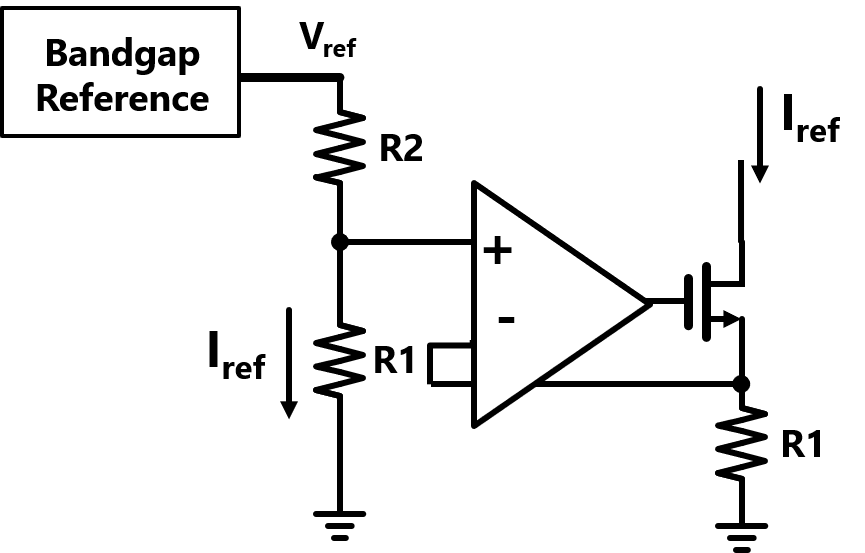
\includegraphics[width=0.5\textwidth]{figs/fig1.png}
  \caption{Bandgap reference current source utilizing voltage-current conversion.}
\label{bandgap}
\end{figure}

\begin{figure*}[!]
\centering
 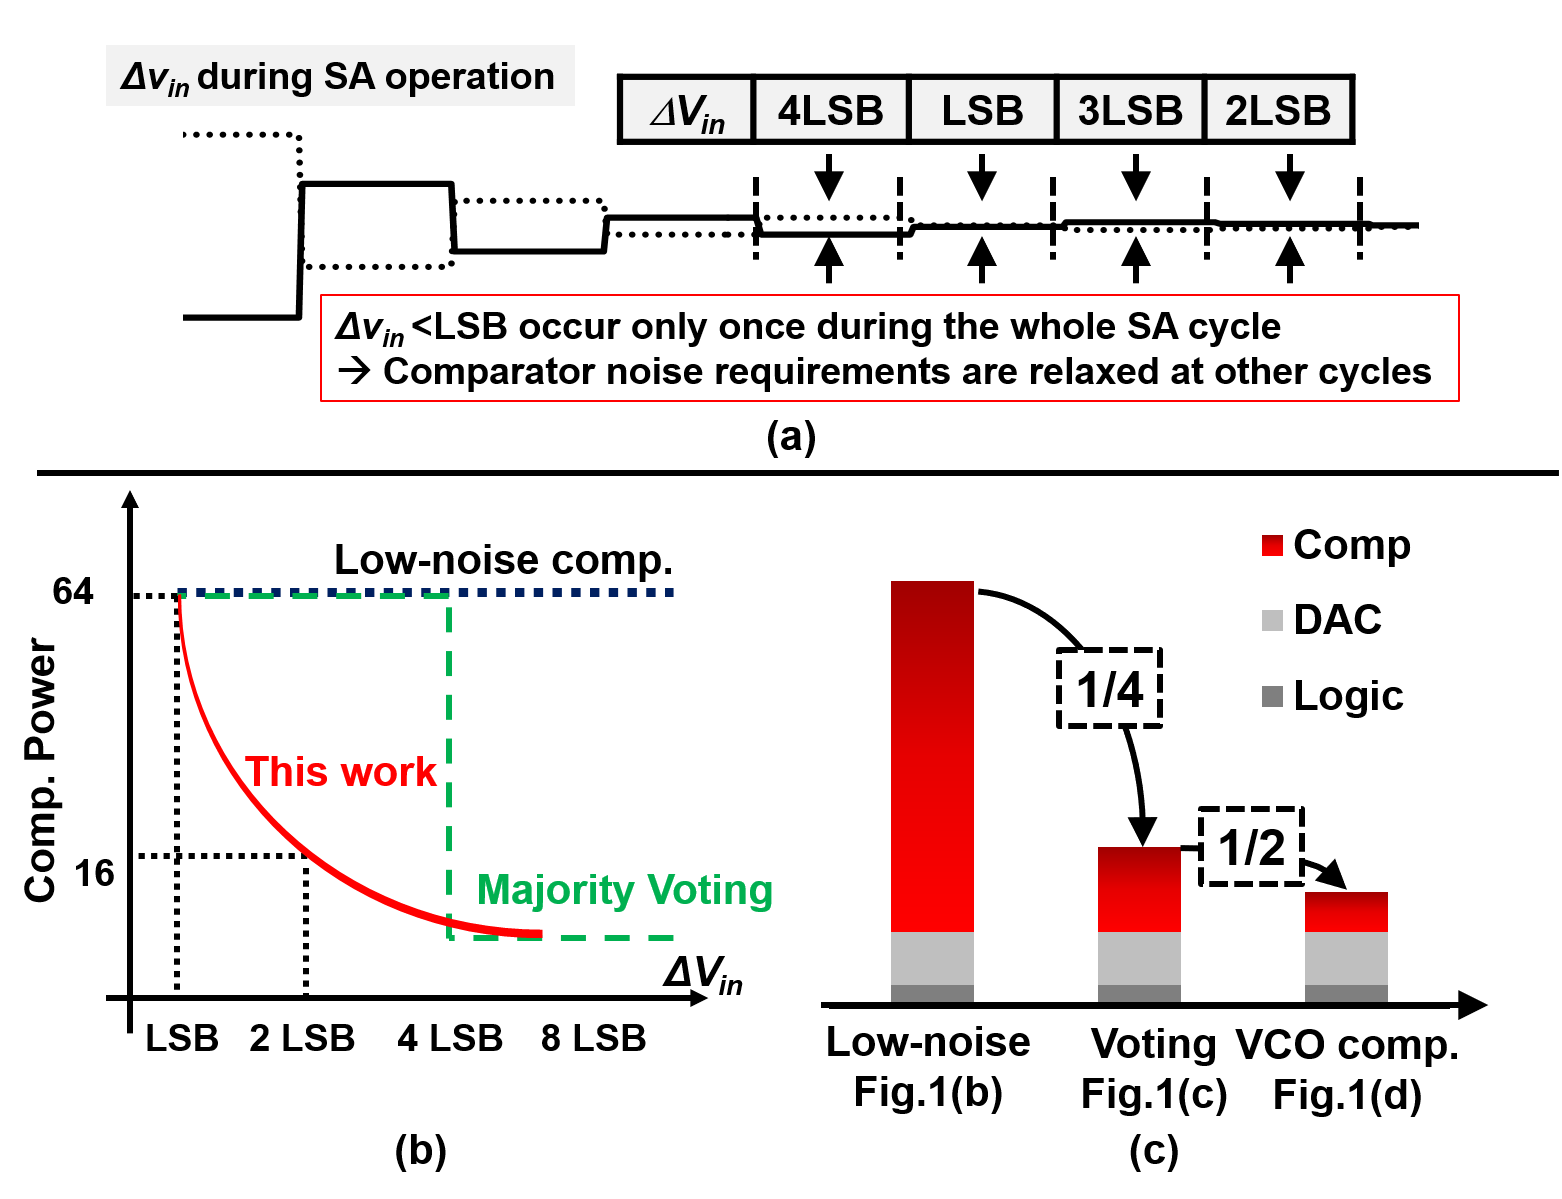
\includegraphics[width=0.9\textwidth]{figs/fig2.png}
  \caption{Block diagram of the TBCS. The current is controlled so that the CSD delay will lock to a half cycle of the CLK. When the delay is locked, the current value will depend on the capacitive load and be decoupled from resistor values, thus realizing a PVT robust current source.}
  \label{fig2}
\end{figure*}

\textbf{Bandgap reference} The BGR is widely used as a current source as shown in Fig.\ref{bandgap}. The BGR generates a robust reference voltage $V_{ref}$ and the reference current $I_{ref}$ is generated by voltage-current conversion as:
\begin{eqnarray}
    \centering
    I_{ref} = \frac{V_{ref}}{R_1 + R_2}
    \label{sar13b}
\end{eqnarray}
The BGR can generate a constant voltage without being affected by environmental variations (temperature, transistor threshold, supply voltage). On the other hand, the resistance values R1 and R2 suffer greatly from process variations, where the resistance values can vary by up to $\pm 40\%$ in the case of poly-resistors. For example, when $I_{ref}$=20uA is targeted, we must expect the max-min current values to be 32uA and 12uA, respectively. Such variations increase the opamp design margin and impacts system power consumption.

\textbf{Adaptive current references} Current sources capable of PVT variations are important for analog products and much research has been undergone. Ref.\cite{chuanyang,ron} utilizes a replica opamp together with a capacitive load, and by directly monitoring the slew rate of the opamp, the current reference is configured to satisfy the target slew rate cancelling the PVT variation effects.
While this method can realize a PVT adaptive current source, a replica opamp is required and significant power and area must be consumed. On the other hand, TBCS can realize a PVT-robust current source using mostly-digital circuits without analog components; the overhead is small.

\textbf{Analog circuit calibration techniques using time information} Ref.\cite{zhu} uses the time information of the reference clock to calibrate analog circuit characteristics. Specifically, the supply voltage is controlled with a DLL and the basic idea is similar to TBCS. Additionally, ref.\cite{kapusta201314b,tomson} uses a DLL to control the delay of an asynchronous SAR clock to optimize the DAC settling timing.
However, these researches aim to calibrate the delay characteristics of the analog circuits. To the best of the author's knowledge, the proposed TBCS is the first approach to suppress the reference current source variation using time information.

%ここまで読んだ

\section{Time based current source (TBCS)}
\subsection{TBCS fundamentals}
A simplified circuit block diagram of the TBCS is shown in Fig.\ref{fig2}. The TBCS requires only a  predetermined frequency clock ($CLK$), such as the sample clock of an ADC, and its components and operation are similar to a Delay-Locked-Loop circuit (DLL) \cite{ sidiropoulos1997semidigital, lee19942, razavi2018delay}. The reference current ($I_{ref}$) is produced, which is fed to the core circuitry (e.g. opamp) and in TBCS $I_{ref}$ is also given to the current-starved-delayline (CSD). The CSD outputs $CLK_{CSD}$, which is a signal appending a delay to $CLK$. The appended delay in $CLK_{CSD}$ is expressed as $N \times t_{DL}$, where the number of stages in the CSD is $N$ and the CSD stage delay is $t_{DL}$. Note that the larger $I_{ref}$ is, the smaller $t_{DL}$ becomes and vice versa. 
Then, phase comparison is performed between $CLK_{CSD}$ and $CLK_B$ (the inverted output of CLK). Given the comparison results, the $I_{ref}$ is controlled so that the delay will converge to the half-cycle time of CLK ($T_D$). Note that frequency references can be finely generated from crystal oscillators, providing a precise reference independent of PVT variations. While loop filters \cite{sidiropoulos1997semidigital} and digital filters \cite{kim20172} are utilized in typical DLLs to generate fine delay, TBCS does not require such filters because its main purpose is to realize a robust current source and not providing precise delays.


\begin{figure}[!]
\centering
 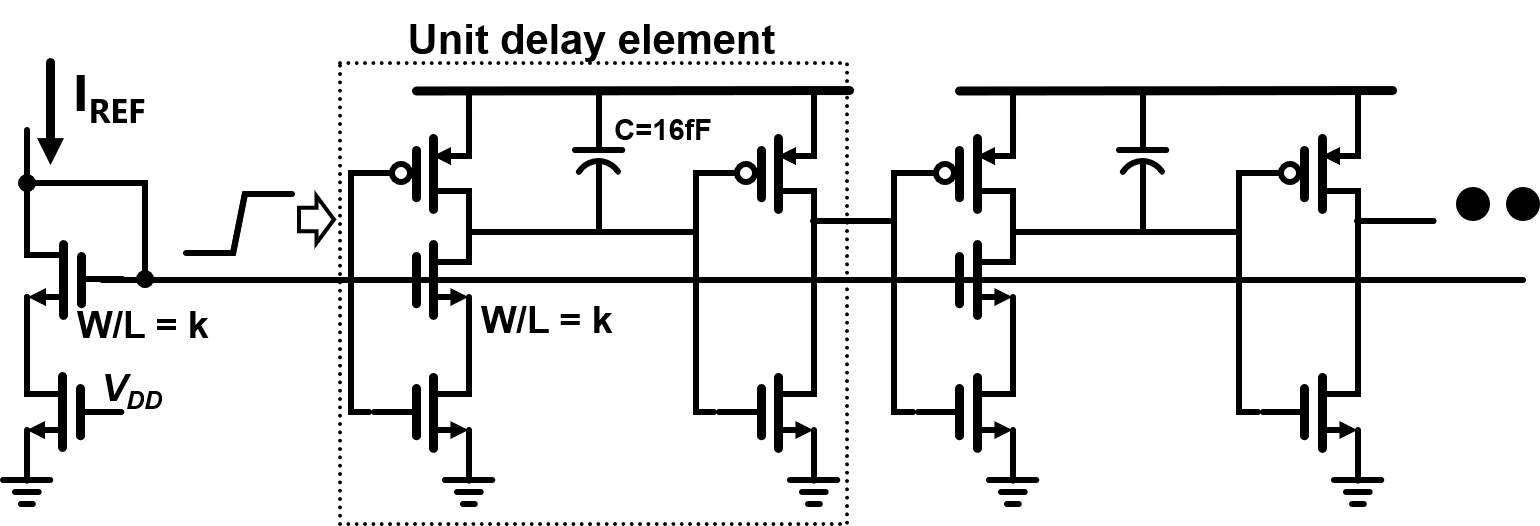
\includegraphics[width=0.5\textwidth]{figs/inv.png}
  \caption{Circuit diagram of the current-starved delayline (CSD).}
\label{inv}
\end{figure}

By further studying the delay characteristics of the CSD, we show that the TBCS is capable of the robust current generation (Fig.\ref{fig2} lower-right).
The circuit diagram of the CSD circuit is shown in Fig.\ref{inv}, consisting of a current-starved inverter(CSI)\cite{mroszczyk2014tunable} driving the capacitive load $C$ and the next-stage inverter. Based on the large-signal characteristics, the CSD unit delay $t_D$ can be expressed as: 
\begin{eqnarray}
    \centering
    t_D = \frac{V_{th}C}{I_{ref}}+t_{inv}
    \label{delay}
\end{eqnarray}
where $V_{th}$ and $t_{inv}$ is the on-threshold and the delay of the next-stage inverter, respectively.  Since the signal is fully propagated by the time the CSI current source enters the triode region, such effect can be neglected from analysis. In eq.(\ref{delay}), if we assume that $t_{inv}$ and $V_{th}$ variation is sufficiently small, $t_D$ will be determined by $C$ and $I_{ref}$. 
Since TBCS converges $t_{DL}$ to a predetermined value, after locking, $I_{ref}$ will become a value corresponding to the capacitance $C$. In advanced CMOS processes, capacitors are significantly less invariant to environmental variations such as voltage, temperature, and mismatch compared to resistors and transistors. Therefore, TBCS can achieve robust current generation independent of environmental variations with delay lock-based configuration.

From eq.(\ref{delay}), the TBCS variation factors are 1) next-stage inverter delay 2) load capacitance variation and 3) $V_{th}$ variation.
Since the delay of the next-stage inverter is one order of magnitude smaller than the CSI delay, its effect is small. On the other hand, the capacitance variation must be small for TBCS to be a robust current source. While metal-insulator-metal (MIM) capacitors have small local mismatches, it is not suitable for TBCS due to its large absolute capacitance variation. On the other hand, metal-oxide-metal (MOM) capacitors have a significantly smaller absolute capacitance variation, making them suitable for TBCS. Moreover, in the next section, we will show that the current drifts due to capacitance and $V_{th}$ variation can help to stabilize the opamp characteristics.

\subsection{PVT adaptive current generation characteristics}
\begin{figure}[!]
\centering
 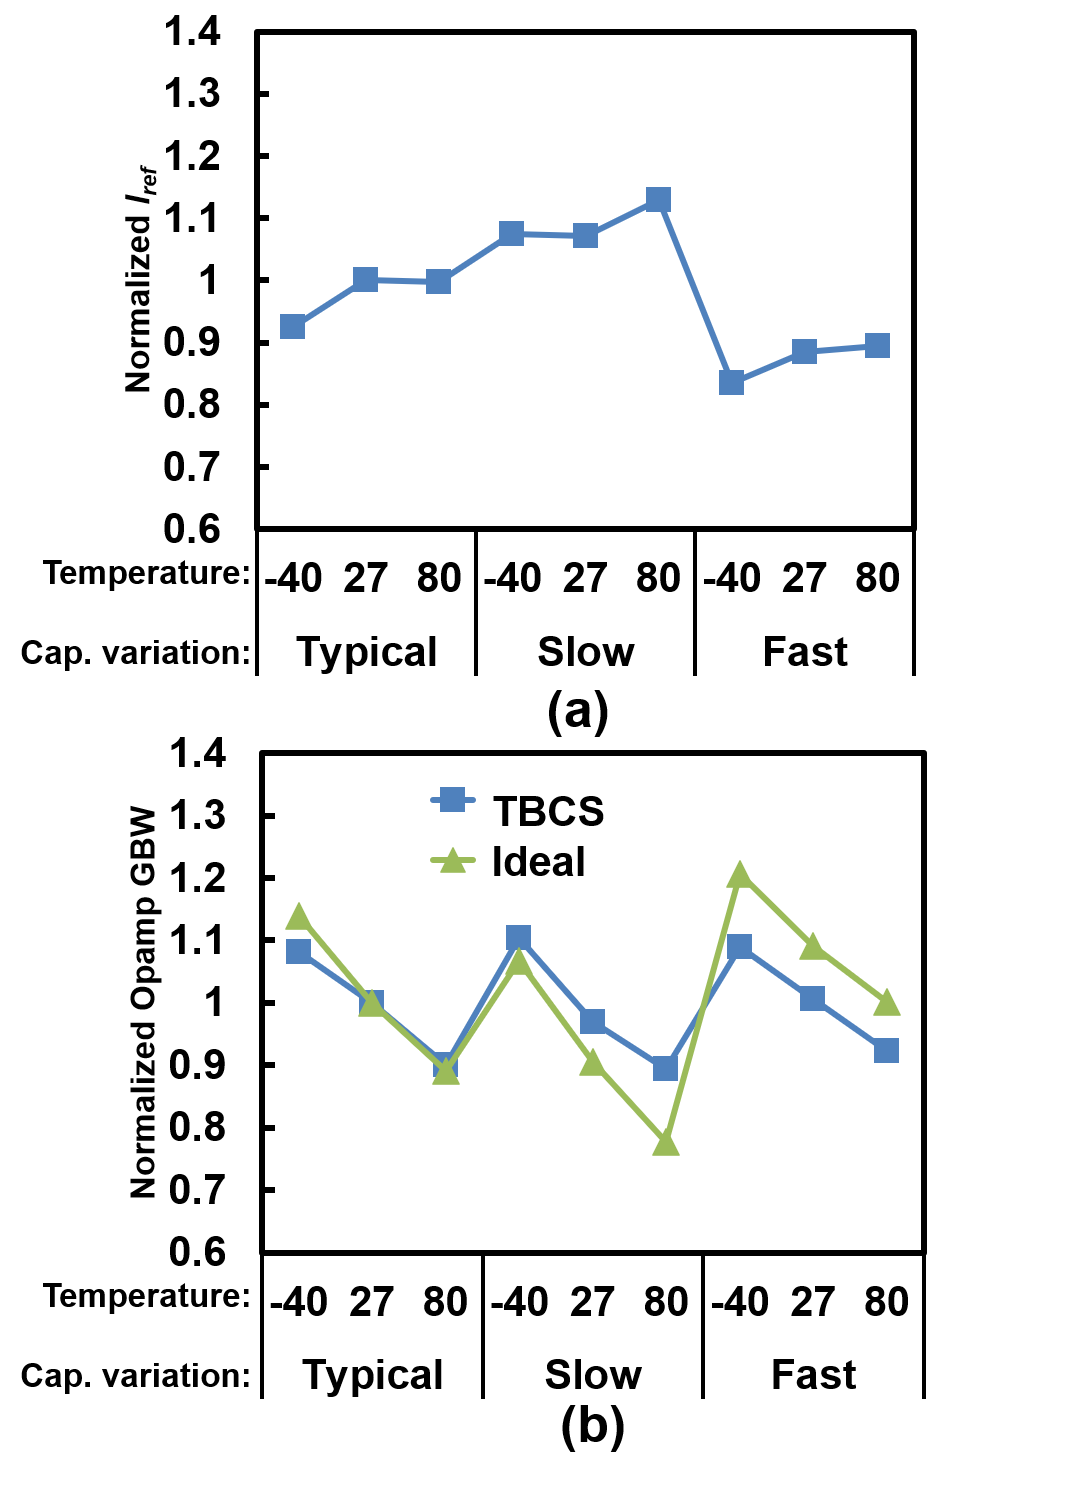
\includegraphics[width=0.5\textwidth]{figs/iref_var.png}
  \caption{(a) Simulation results of the TBCS $I_{ref}$ under capacitor manufacturing variations. "Slow" conditions indicate variations with increased capacitance and \textit{vice versa}.  (b) Simulation results of the opamp GBW biased by TBCS and ideal current source under the same variations, respectively.}
\label{cvar}
\end{figure}

While the TBCS is decoupled from resistor variation, the capacitor and $V_{th}$ variation causes current drifts since $T_{DL}$ is determined by the capacitor charging time. Interestingly, the current drift due to the capacitance variation militates to improve the opamp PVT tolerance.
From eq.(\ref{delay}), as $C$ increases, $I_{ref}$ will increase, and conversely, as $C$ decreases, $I_{ref}$ decreases. Such characteristic is undesirable from the viewpoint of a \textit{constant} current source. On the other hand, it is important to note that when such capacitance variation occurs, the load capacitance of the opamp will increase/decrease as well. As the load capacitance increases, the gain-bandwidth (GBW) of the opamp degrades; however, the TBCS \textit{adaptively} increases the current to compensate for the degraded GBW. Thus, the TBCS will help to keep the opamp GBW constant through PVT variations. $V{th}$ variation has a similar effect: under "slow" conditions where $V_{th}$ increases, $I_{ref}$ increases to compensate for the slowdown of the opamp.

To further analyze this effect, we perform extensive simulations, where Fig.\ref{cvar}(a) and (b) show the generated TBCS current ($I_{ref}$) and opamp GBW under capacitance variation, respectively. Here, a simple two-stage differential opamp biased via TBCS was utilized. In the "slow" conditions (larger capacitance), the $I_{ref}$ increases by about 10-15\%, which compensates for the opamp GBW degraded by the increased load capacitance. Interestingly, due to the adaptive current generation, TBCS can maintain opamp GBW constant through variations than an ideal current source. Under "fast" conditions, the $I_{ref}$ is reduced, but the effect on GBW is small because the opamp load is also reduced. Thus, TBCS reduces the power consumption while maintaining the required opamp GBW. 

In general, mass-produced chips are designed to meet the critical performance (e.g. opamp GBW) even under the worst variations. Therefore, if we can supress GBW degradation under the worst condition, the design margin can be  reduced to improve the system power consumption. In Fig.\ref{cvar}(b), the GBW under the worst condition is improved by 13\% with TBCS over the ideal current source, proving that TBCS contributes to the design margin reduction.

\subsection{Varying CLK input frequency}
\begin{figure}[!]
\centering
 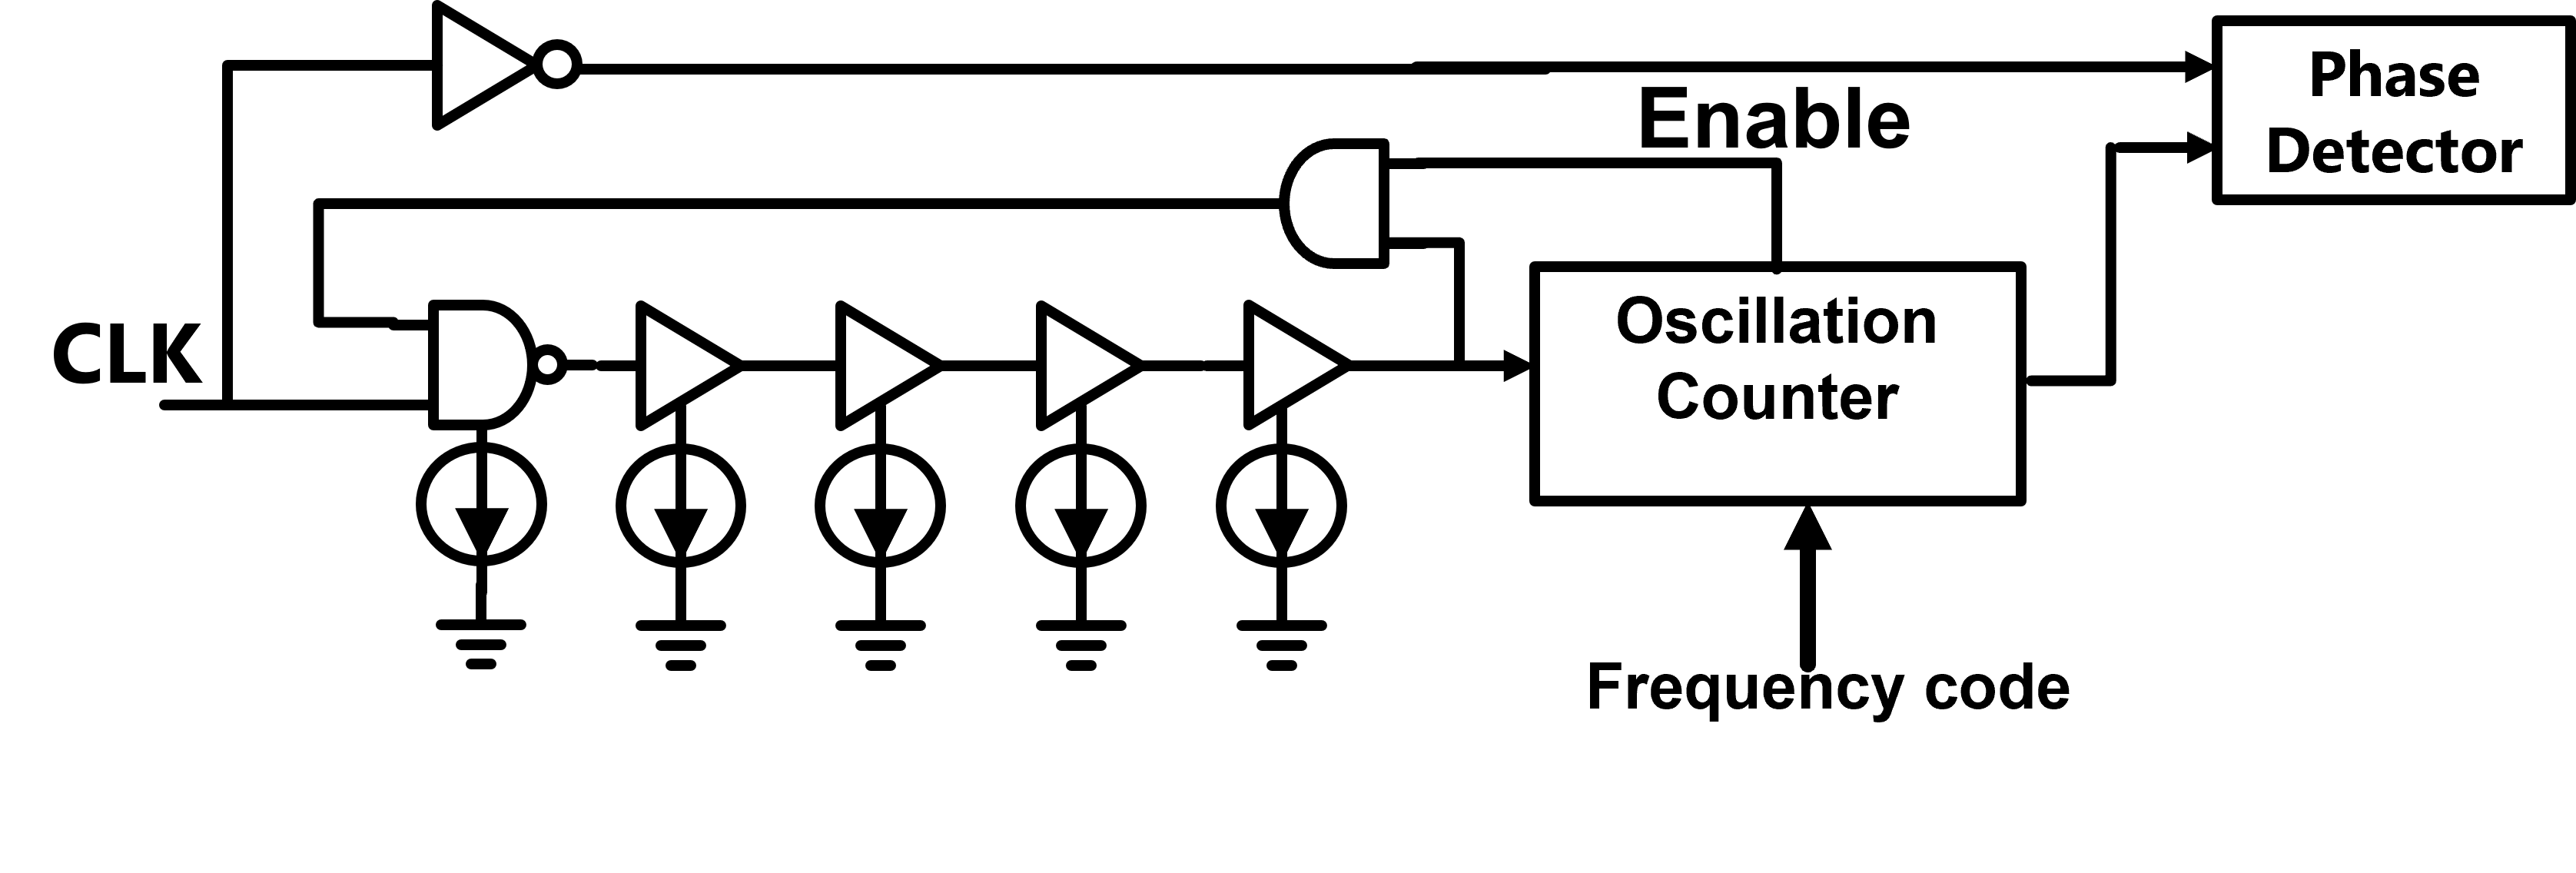
\includegraphics[width=0.5\textwidth]{figs/osc_tbcs.png}
  \caption{Circuit diagram of TBCS supporting multiple input frequencies. The use of oscillation  counter makes it possible to lock to the same $I_{ref}$, as long as the input frequencies are integer multiples of each other.}
\label{counter}
\end{figure}

In this design, the CSD is designed with the assumption that the clock frequency is fixed to 80MHz. Since we are considering a wireless frontend as an application, other operating frequencies such as 20MHz and 40MHz can be considered as TBCS input candidates. %Without any elaborations, the $I_{ref}$ will simply be stuck to the minimum value. If the opamp can function with such a current, then additional circuitry will not be required.
%There are also cases where a constant $I_{ref}$ is required regardless of the frequency. 
Here, we will show some additional design ideas to realize TBCS with multiple input frequencies. If the candidate clock frequencies have a relationship of integral multiples (common for wireless receiver ADCs), a constant current can be generated by oscillating the CSD multiple times as Fig.\ref{counter}. For example, when the input clock is 1/4 of the design frequency (20MHz), the current source can be locked at a state close to 80MHz by oscillating the CSD four times using a counter to generate a constant current. Note that the input frequency state must be given to the counter for operation.

%またCSDのM段目出力を用いて位相比較を行うようことでfractional周波数においても電流生成が可能である。カウンタを制御するための周波数情報は前もって入力する必要はあるが一般的にPLLはそのような情報を元に周波数を生成しているため情報を得るのは容易い。

\section{Circuit Implementations}
\subsection{Control circuit}
\begin{figure}[!]
\centering
 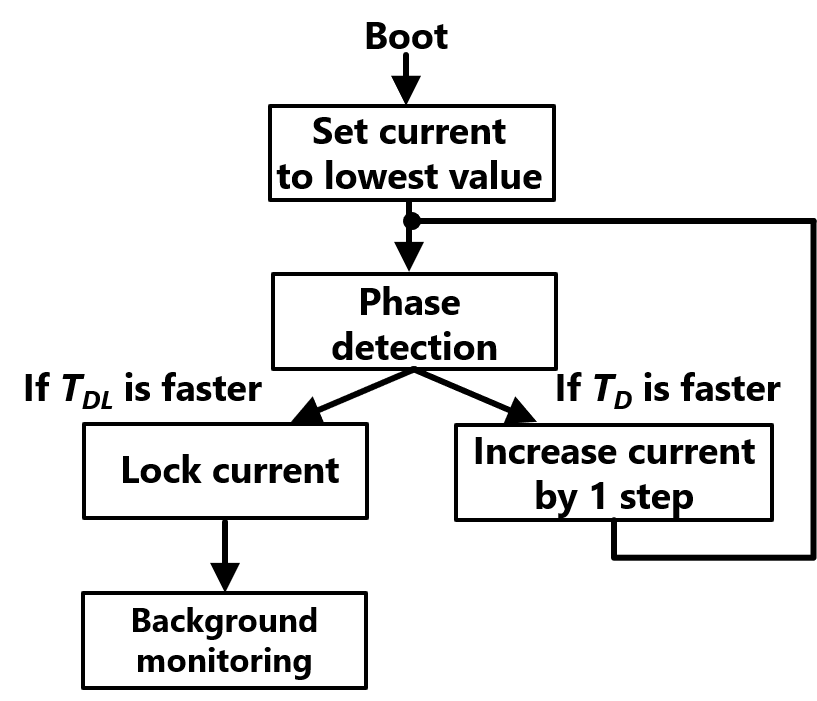
\includegraphics[width=0.5\textwidth]{figs/flowchart.png}
  \caption{TBCS control flowchart.}
\label{flow}
\end{figure}
Firstly, the basic control flow of TBCS is explained in detail using Fig.\ref{flow}. When the power is turned on, the current source is set to output the lowest $I_{ref}$. Then, the optimal current code is searched by increasing the code step by step. Since $I_{ref}$ is small at the beginning, $T_{DL}$ is prolonged and the phase detector judge that $T_D$ arrives early and $I_{ref}$ is increased by one step. This procedure is repeated, and once $T_{DL}$ arrives earlier, the current is "locked" and TBCS enters the background tracking mode.

Since this control method is a simple bang-bang control, maximum of $2^N$ cycles are required to converge ($N$ is the number of bits in the configurable current source). For example, if we utilize successive approximation, we can achieve faster convergence. However, it may not be possible to track the environment drifts during the locking procedure (e.g. sharp voltage drifts).

\subsection{Phase detector}

\begin{figure}[!]
\centering
 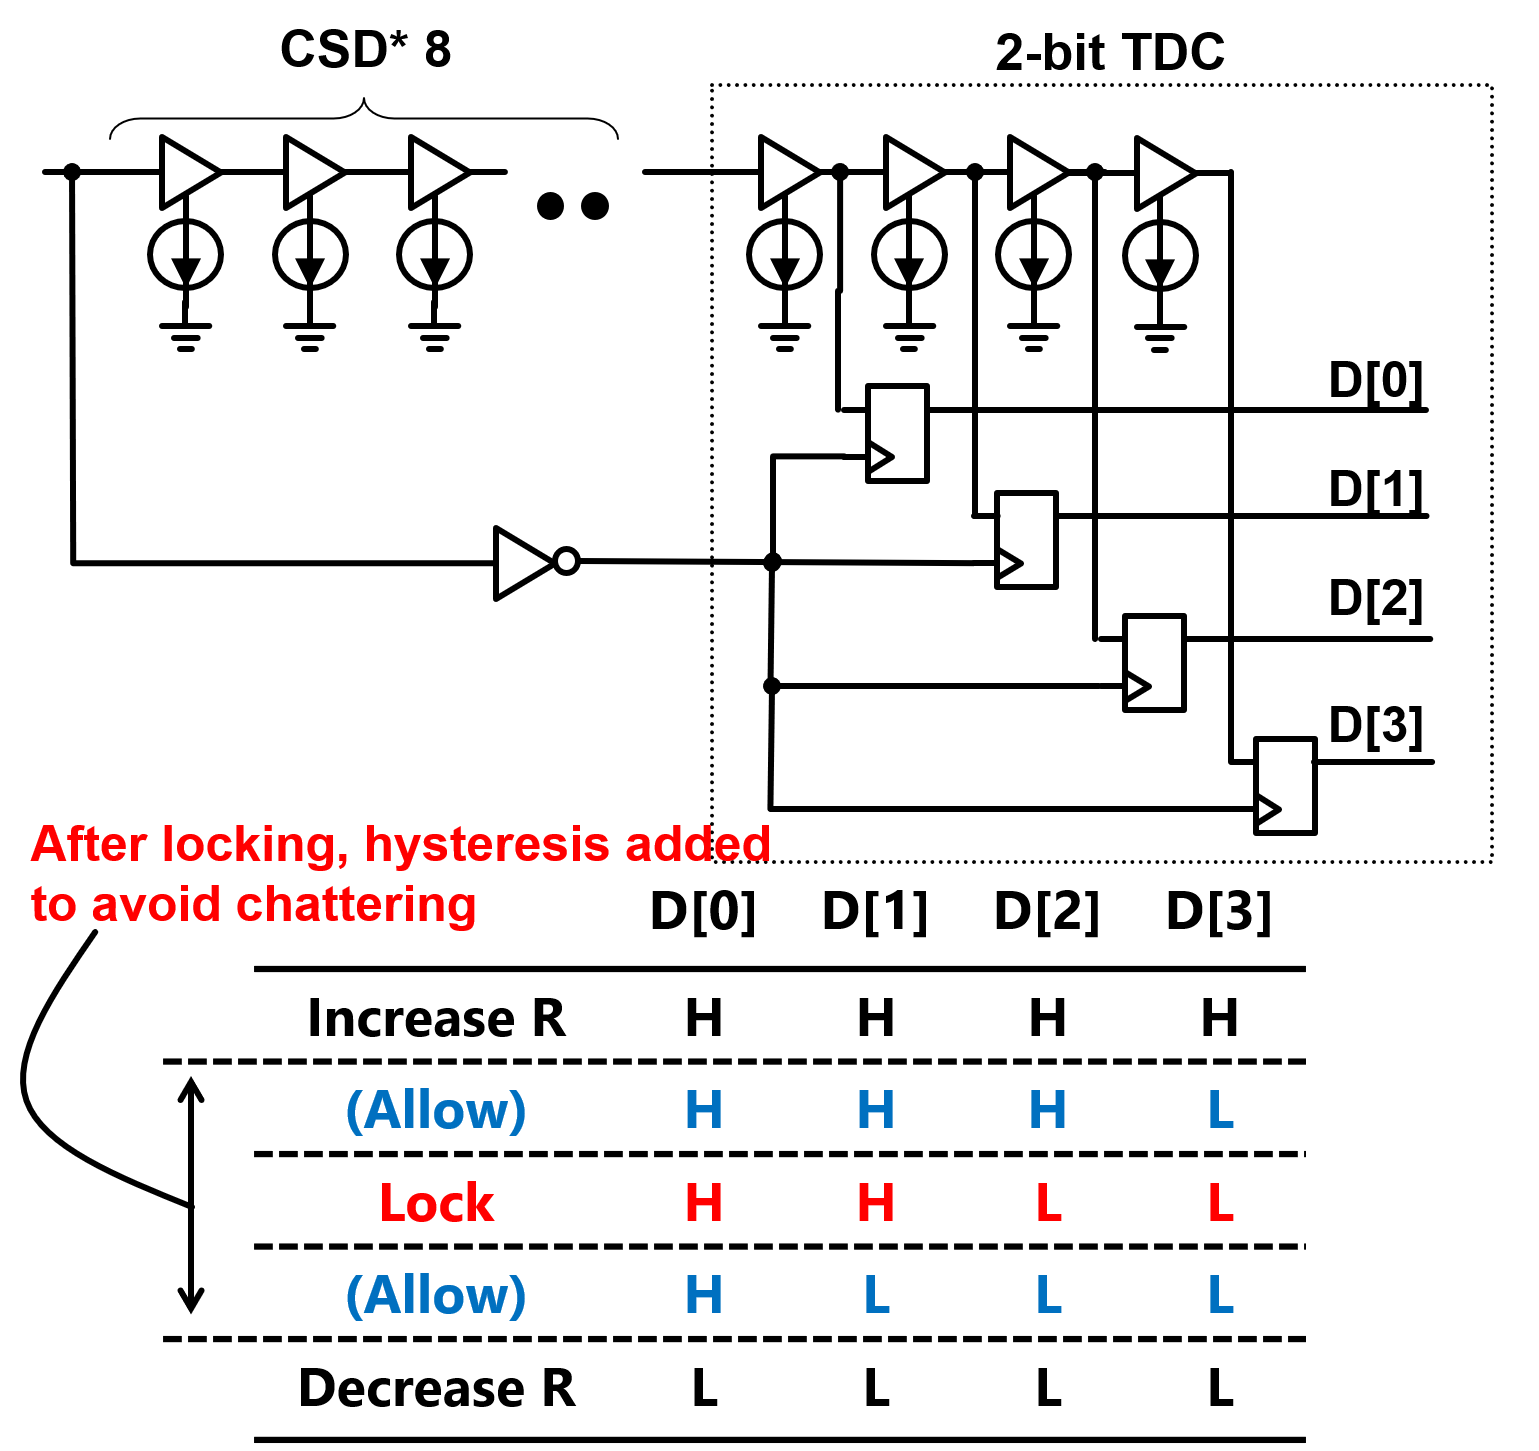
\includegraphics[width=0.5\textwidth]{figs/tdc.png}
  \caption{Background monitoring control of TBCS utilizing a 2-bit TDC circuit.}
\label{tdc}
\end{figure}

\begin{figure}[!]
\centering
 
\includegraphics[width=0.5\textwidth]{figs/chattering.png}
  \caption{Timing chart showing the chattering effects.}
\label{chattering}
\end{figure}

Next, we will discuss the implementation of the phase detector. While an 1-bit TDC can be easily realized with a single flip-flop, there is a possibility of code flapping (chattering) which is illustrated in Fig.\ref{chattering}. If $I_{ref}$ is increased in the first phase cycle (code 14 to 15), the delay become smaller than $T_D$ in the next phase comparison. Then, $I_{ref}$ will be reduced in the next cycle reflecting the comparison result (codes 15 to 14) and such chattering may cause unwanted spurs in the SC circuit. While chattering can be prevented by fixing the control code after the current is locked, but TBCS will lose the ability to track PVT drifts.

In our design, we utilize a 2-bit TDC as the phase detector to prevent chattering and  provide PVT drift tracking (Fig.\ref{tdc}).
Once the current is locked, the TBCS enters the background monitoring mode to track long-term environmental variations.  As shown in the table of Fig.\ref{tdc}, the current code is not updated except when all the D[0:3] bits transitions to High or Low, which prevents chattering but can respond to long-term environmental changes. Note that before locking, only bit D[1] is used for control (identical to 1-bit TDC), and after locking, the full 2-bit output D[0:3] is utilized.

\subsection{R-DAC based current generator}
\begin{figure}[!]
\centering
 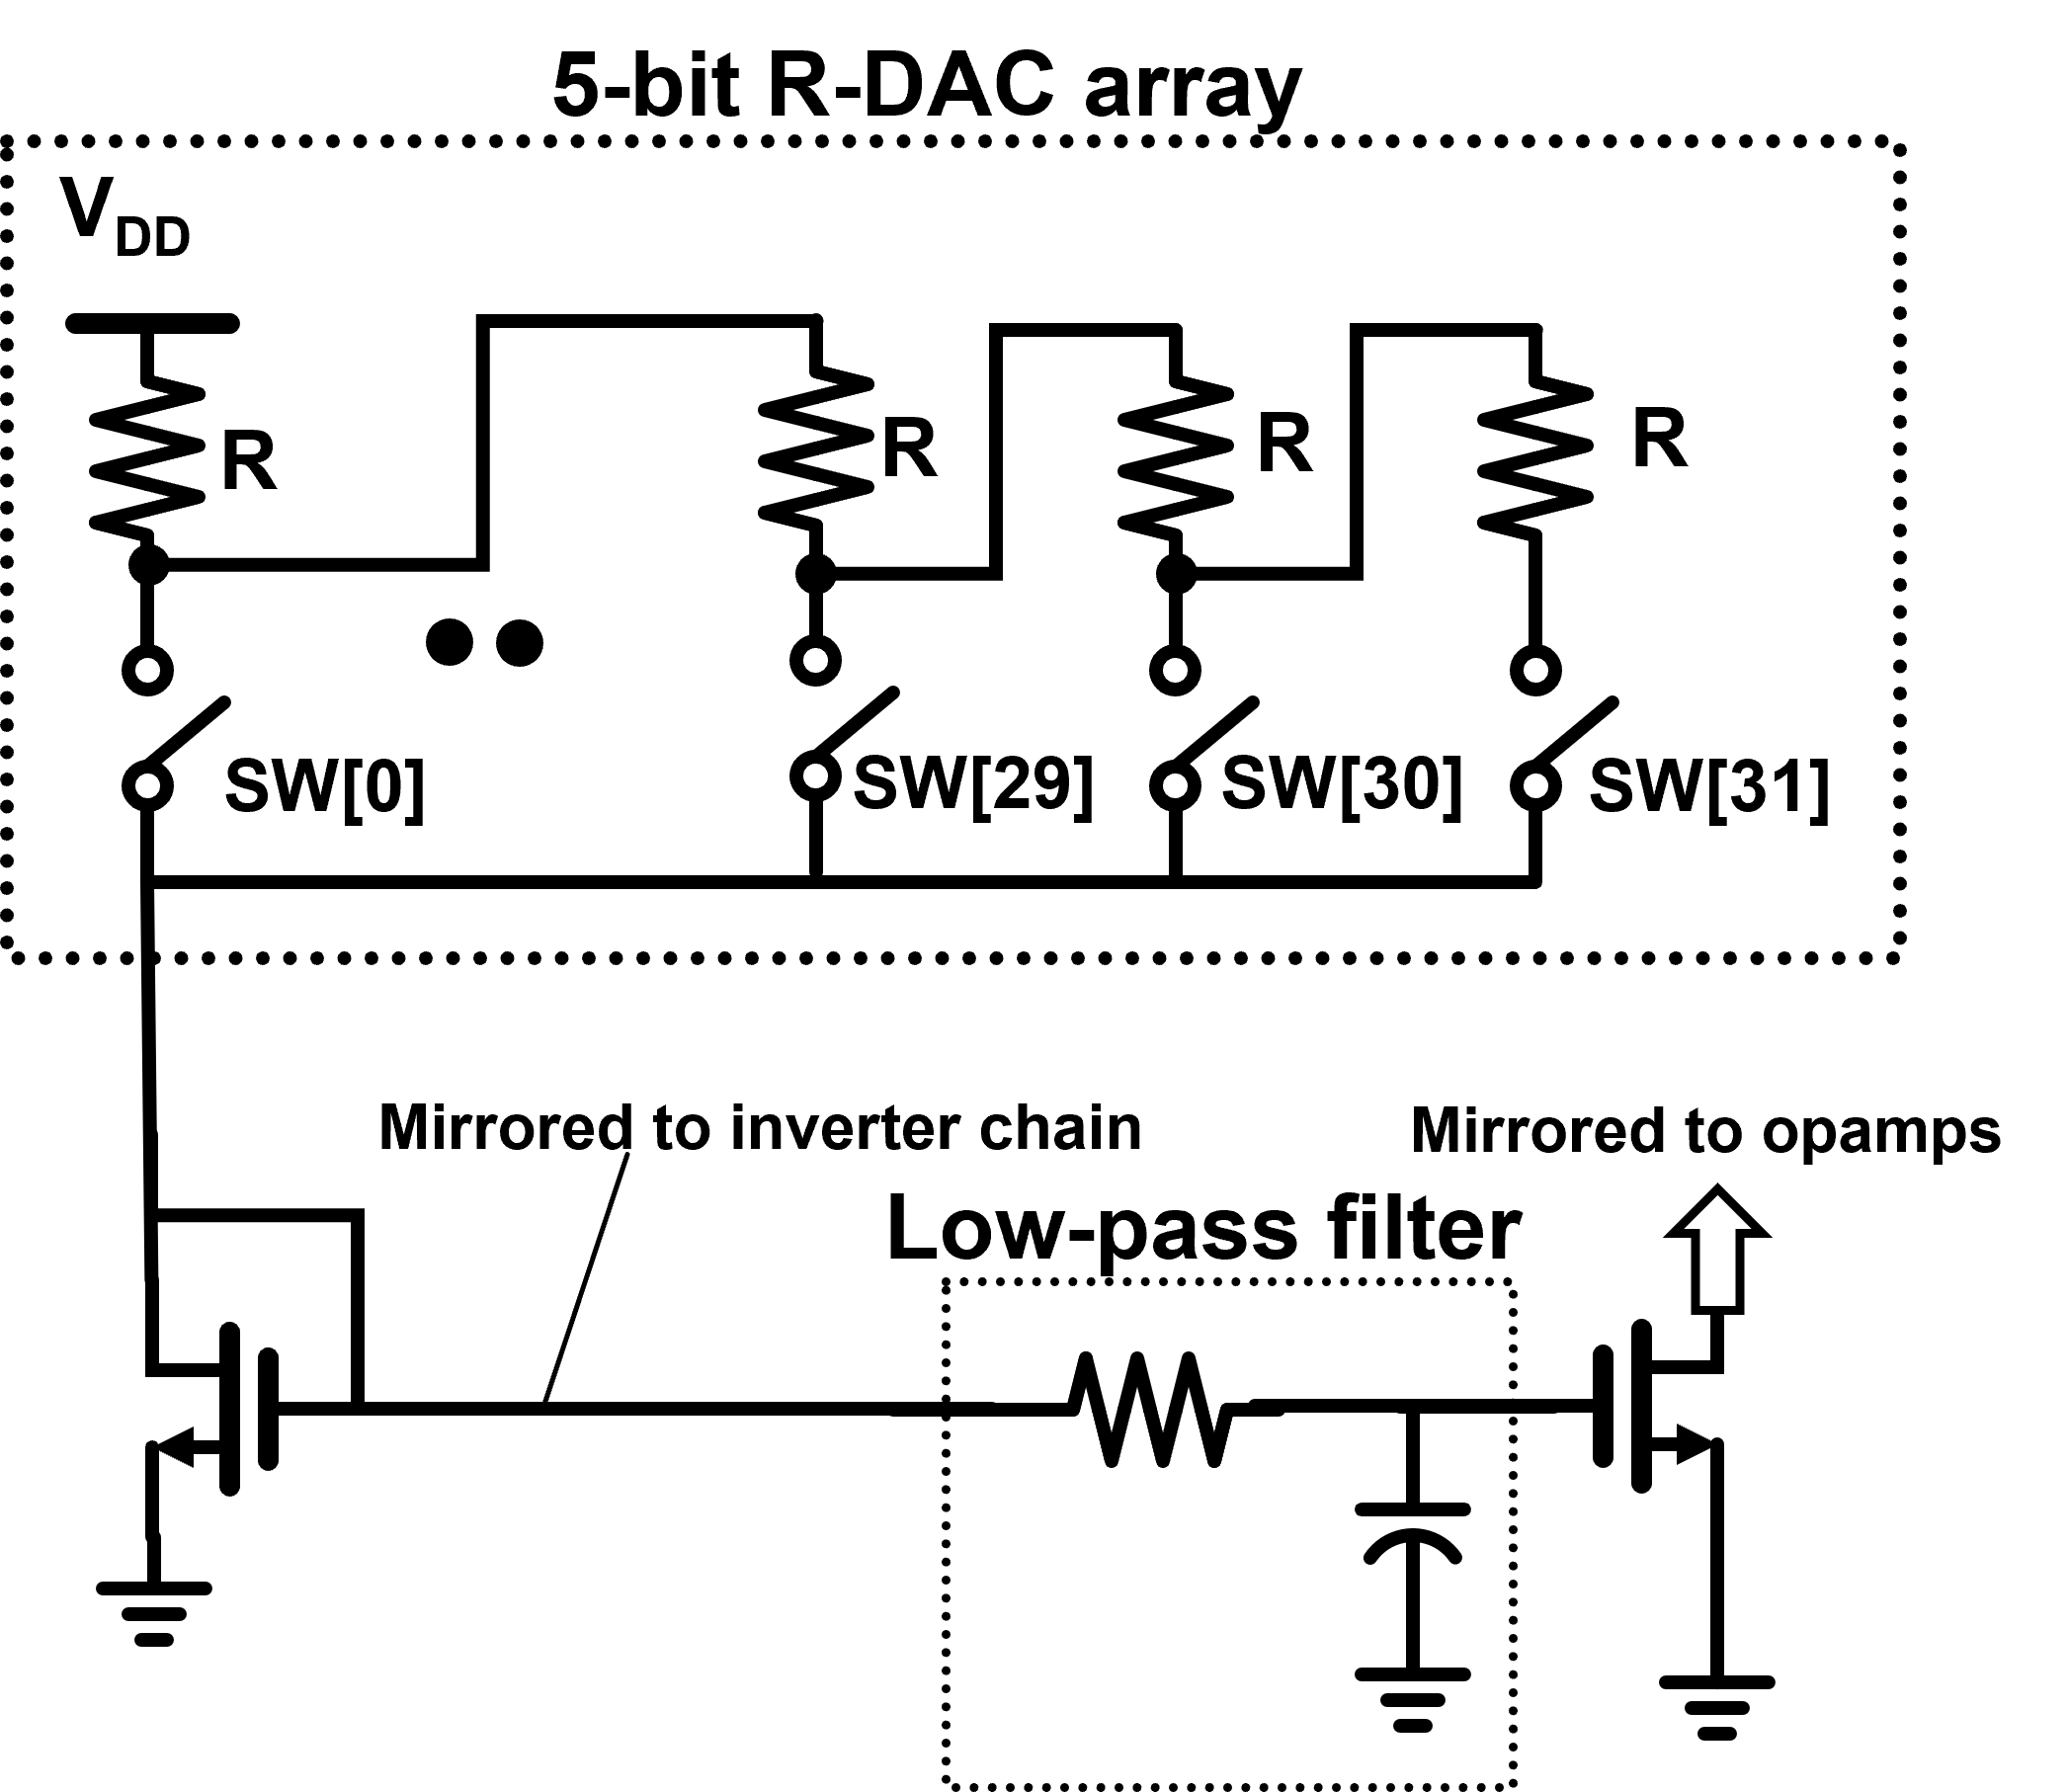
\includegraphics[width=0.5\textwidth]{figs/rdac.png}
  \caption{Circuit diagram of 5-bit R-DAC and low-pass filter.}
\label{rdac_sche}
\end{figure}

The circuit diagram of the R-DAC which constructs the variable reference current source is shown in Fig.\ref{rdac_sche}. The generated current $I_{ref}$ is decided by configuring the resistance value of the R-DAC as:
\begin{eqnarray}
    \centering
     I_{ref} = \frac{V_{DD}}{R_{NMOS}+R_{DAC}}
    \label{iref_eq}
\end{eqnarray}
The R-DAC is controlled by a one-hot digital code (SW[0:31]): when SW[31] is high, the resistance takes the maximum value of 32R and the lowest value R at SW[0]. In TBCS, the R-DAC design is the most critical factor. Specifically, the R-DAC must be designed to satisfy the following two points: (1) whether the accuracy of the generated current is sufficient and (2) whether the target current value can be generated even under PVT variations.

\begin{table}[]
\centering
 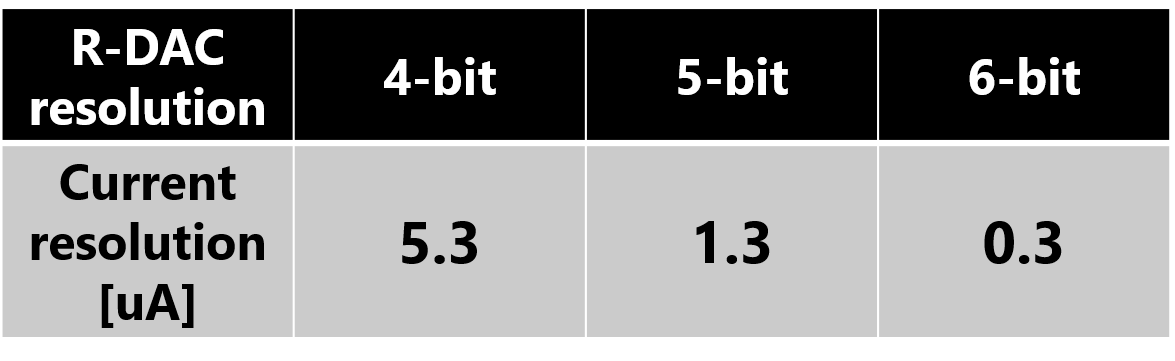
\includegraphics[width=0.4\textwidth]{figs/rdac_table.png}
  \caption{Generated current resolution when using 4, 5, and 6-bit R-DACs. The simulation is done with unit resistance = 4k$\Omega$.}
\label{rdac_table}
\end{table}

First of all, the R-DAC resolution directly couples to the generated current precision as shown in eq.(\ref{iref_eq}). Table \ref{rdac_table} summarizes the simulation result of the $I_{ref}$ resolution when the R-DAC resolution was varied from 4, 5 to 6 bits. In simulations, we adapt the current differential of the center code for simplicity. The 4-bit R-DAC had a step of 5uA, which is too large for our design. On the other hand, the 5-bit R-DAC had a step of 1.3uA, which is sufficient precision.

\begin{figure}[!]
\centering
 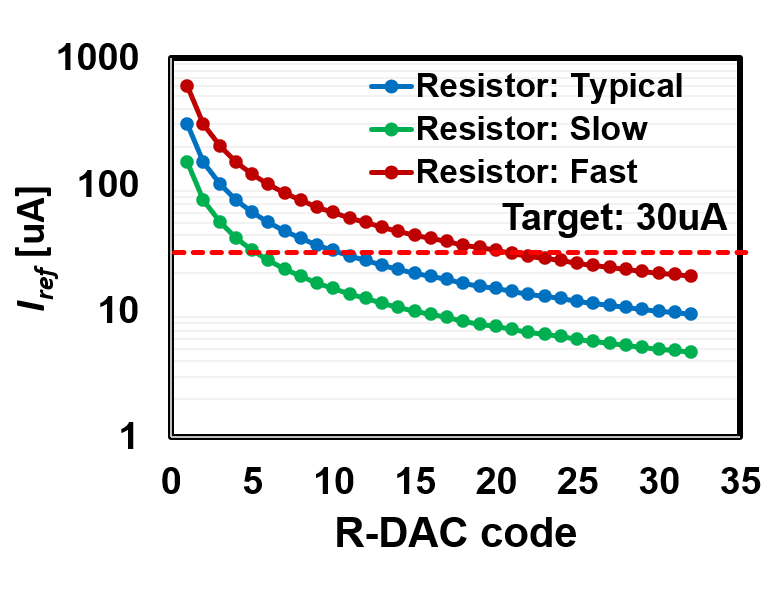
\includegraphics[width=0.5\textwidth]{figs/rdaccode.png}
  \caption{Simulation results of R-DAC code versus generated current under resistance variation.}
\label{rdac_pvt}
\end{figure}

In addition, we need to check if the TBCS can lock to the target current even with resistance variation. The DAC code vs. $I_{ref}$ with resistance variation is plotted in Fig. \ref{rdac_pvt}. It can be seen that the target $I_{ref}$= 30uA can be covered in all conditions. If the resistance variation is too large to cover the target $I_{ref}$, it is necessary to increase the R-DAC resolution and make the resistor range wider.

Moreover, unnecessary spurious components may be propagated to the operational amplifier caused by resistor switching. To remove such unwanted components, a low-pass filter is configured (Fig.\ref{rdac_sche}) with passive devices to remove the switching component from the opamp bias.

\subsection{Current starved delay-lines}

Finally, we describe the current starved delay-line (CSD) shown in Fig.\ref{inv}. While resistance mismatch affects $I_{ref}$ in conventional current sources, the effect of resistance mismatch is small in TBCS due to the delay-locking feature. However, the CSD delay time variation has an adverse effect on $I_{ref}$.
If we denote the delay mismatch of the single delayer as $var$, the overall variation of the $N$-stage CSD increases to $var \times \sqrt(N)$. However, since the signal component also become  $N$ times larger, the variation is mitigated to $\frac{1}{\sqrt(N)}$.

While jitter is also an important design factor in DLLs, the effect is small in TBCS. Since the jitter is sufficiently small compared to the total delay and TBCS uses hysteresis after locking, the jitter effect can be neglected.

\section{Measurement and simulation analysis}
\begin{figure}[!]
\centering
 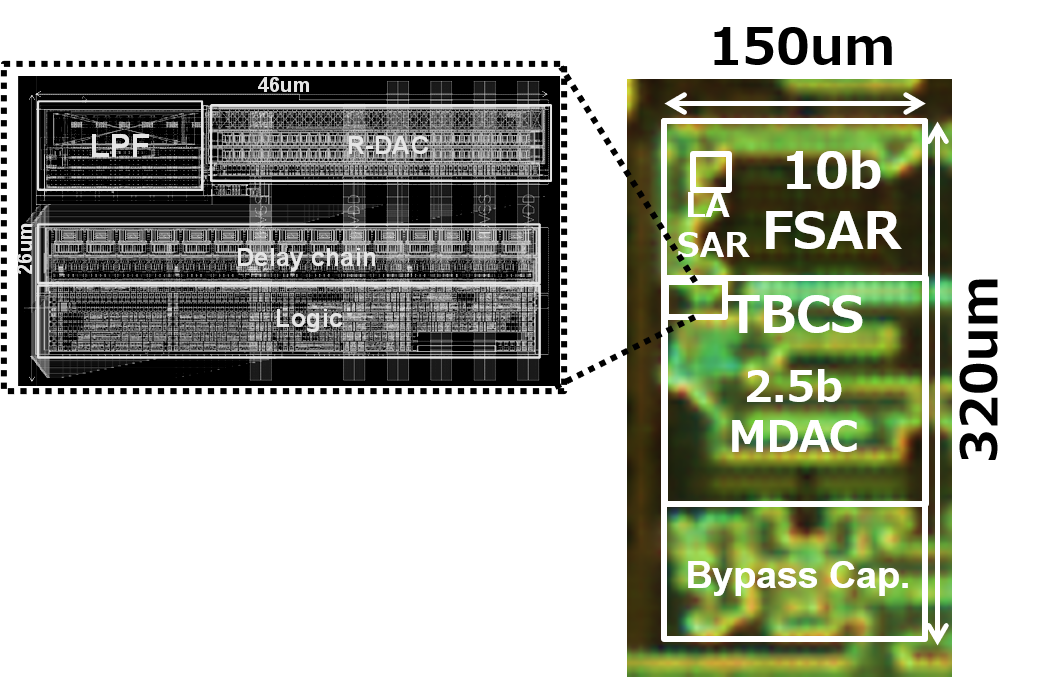
\includegraphics[width=0.5\textwidth]{figs/chip.png}
  \caption{Chip photo and performance summary.}
\label{chip}
\end{figure}

\begin{figure}[!]
\centering
 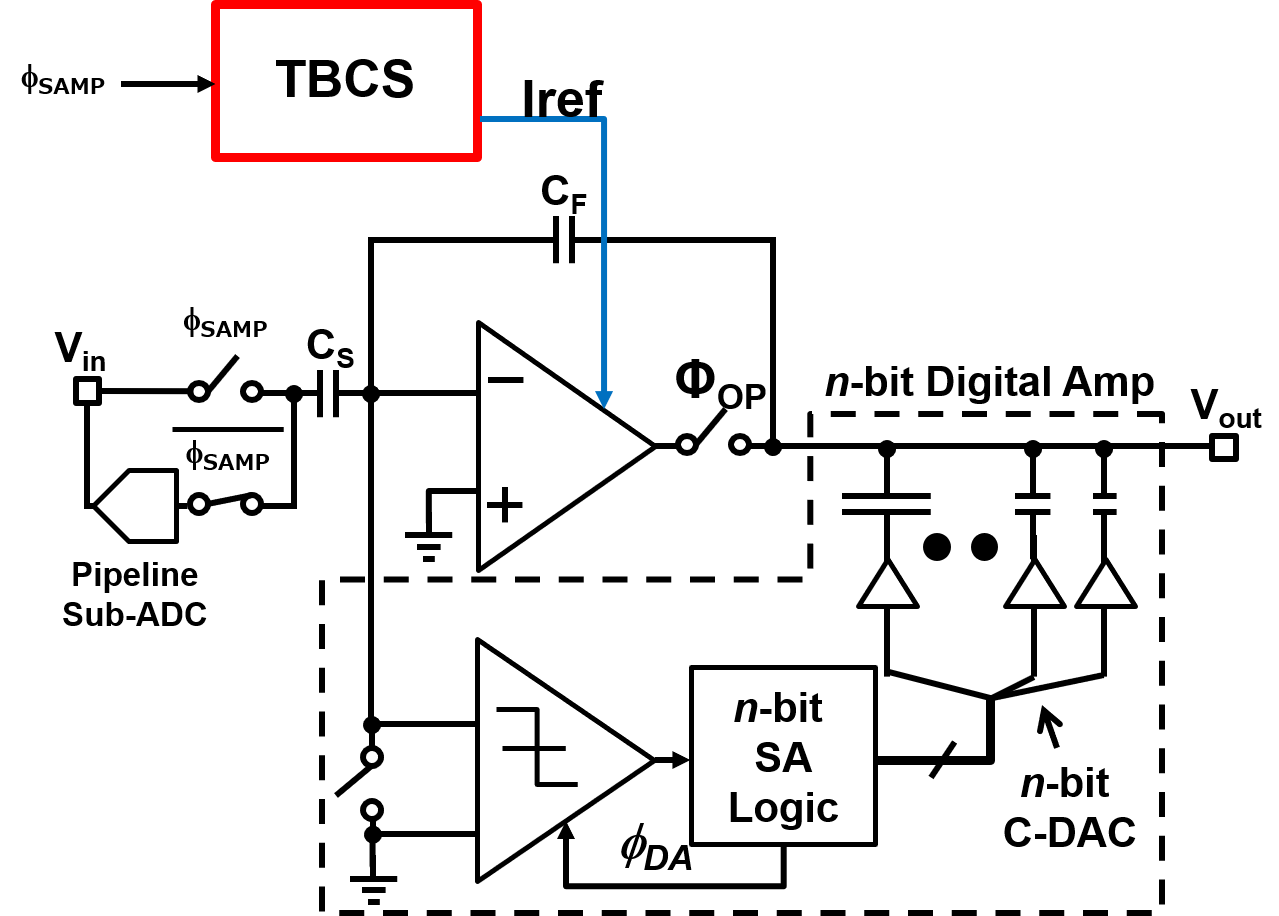
\includegraphics[width=0.5\textwidth]{figs/switchcap.png}
  \caption{Circuit diagram of the SC circuit with integrated TBCS.}
\label{scap}
\end{figure}

\begin{figure}[!]
\centering
 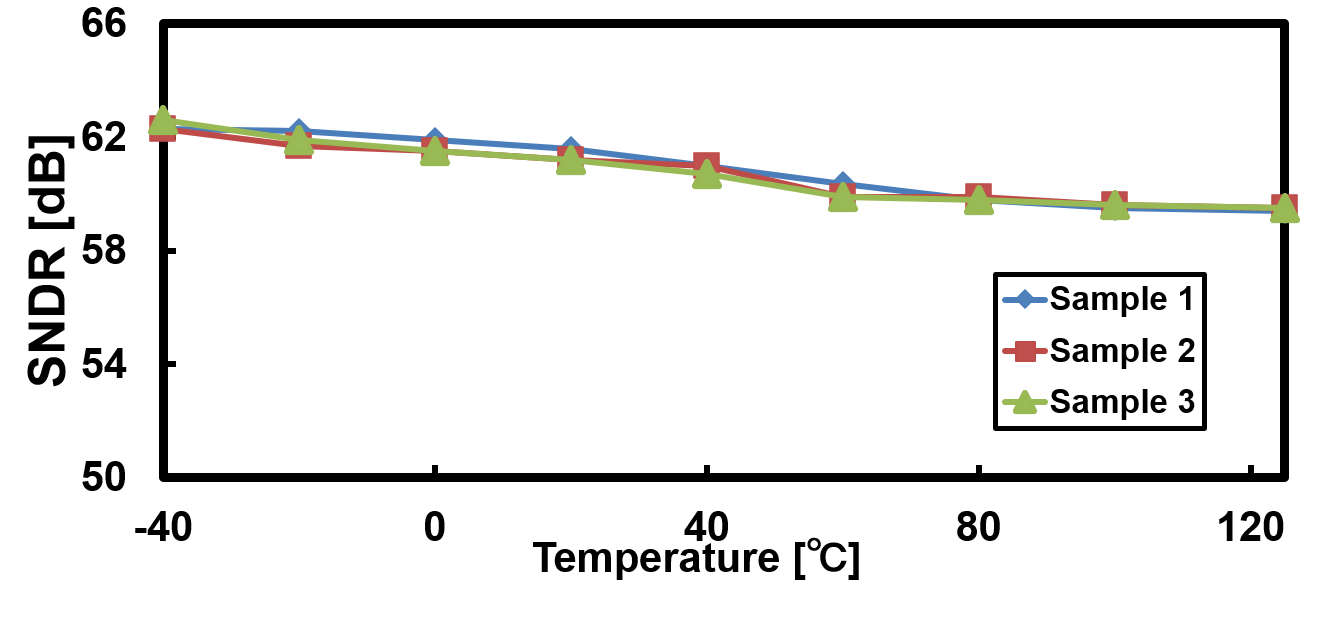
\includegraphics[width=0.5\textwidth]{figs/sndr.png}
  \caption{SNDR measurement results of TBCS integrated ADC.}
\label{sndr}
\end{figure}

\begin{figure}[!]
\centering
 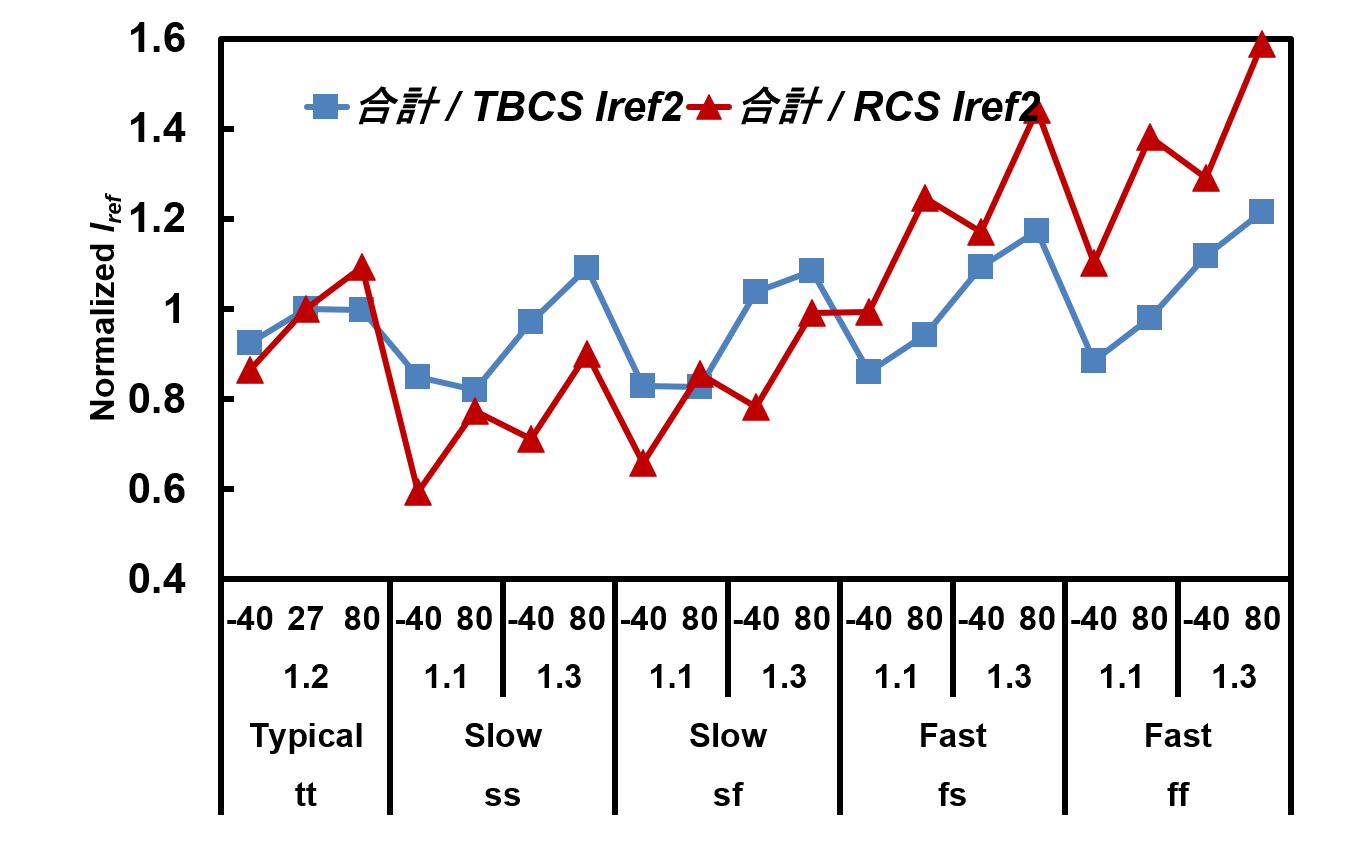
\includegraphics[width=0.5\textwidth]{figs/pvt.png}
  \caption{Simulation result of the TBCS and BGR current source $I_{ref}$ under PVT variations, respectively.
}
\label{iref_pvt_both}
\end{figure}

\begin{figure}[!]
\centering
 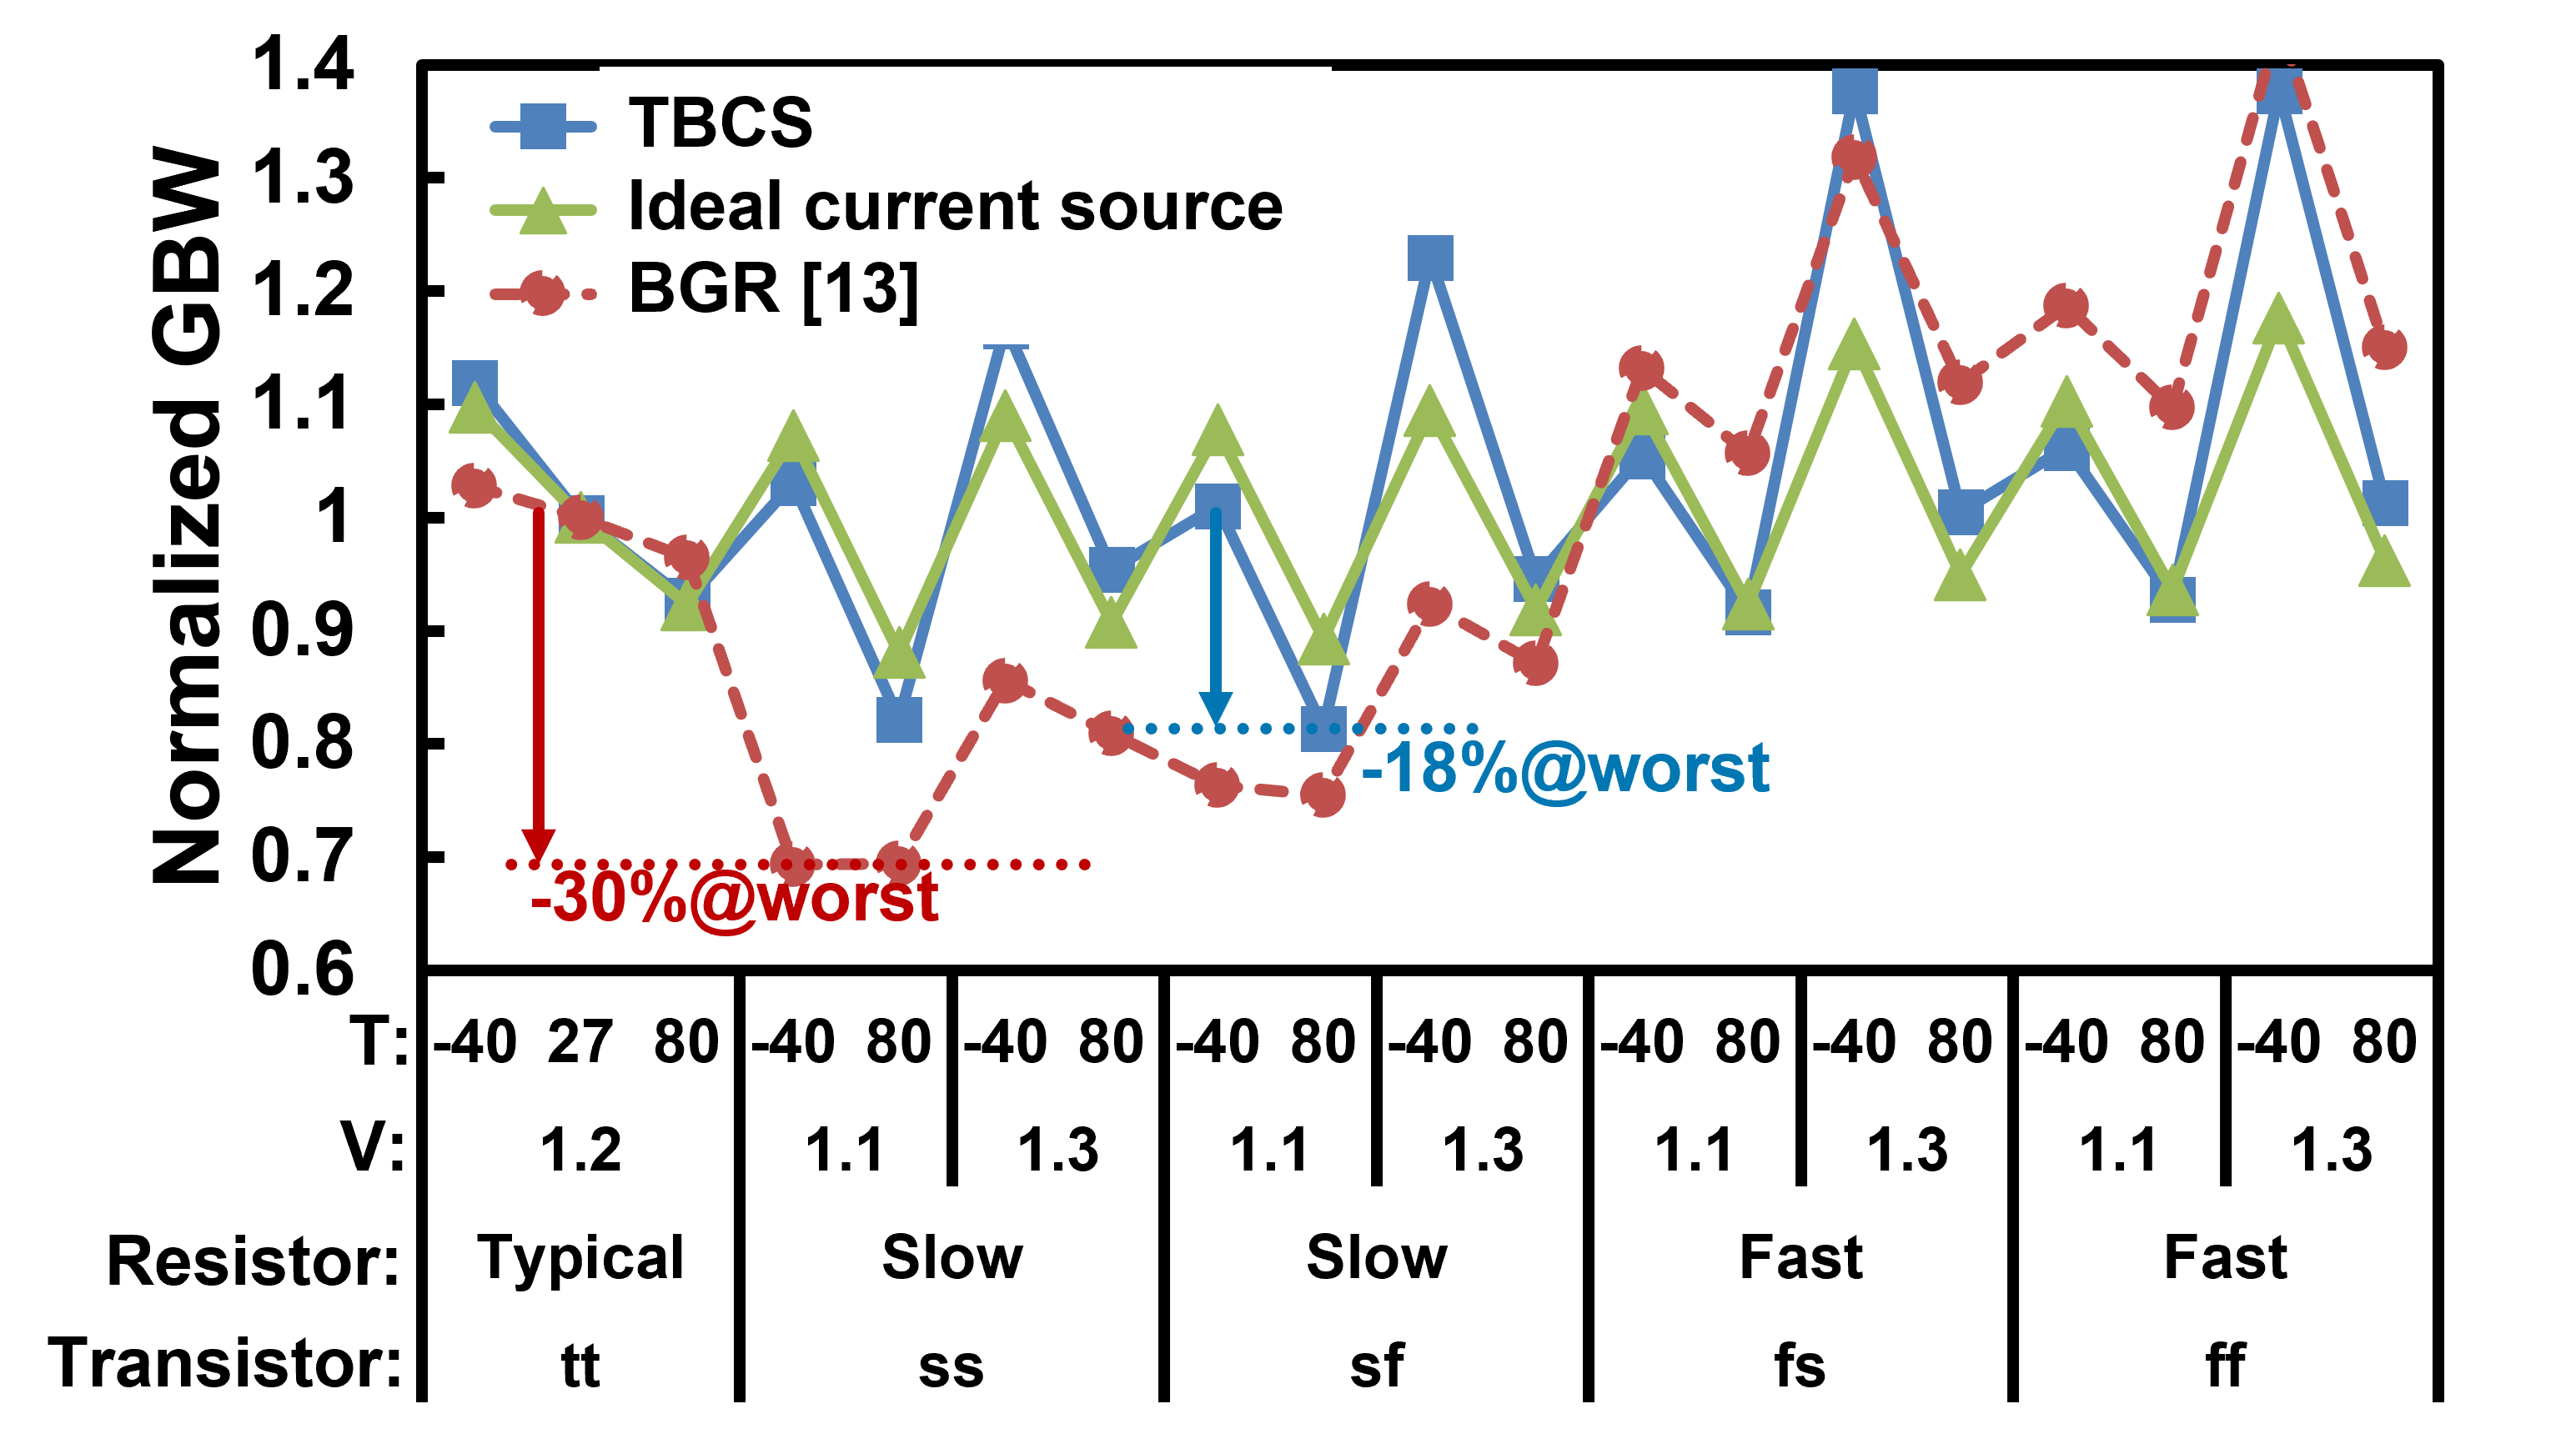
\includegraphics[width=0.5\textwidth]{figs/pvt_gbw.png}
  \caption{Simulation result of the opamp GBW biased with TBCS, ideal and BGR current source $I_{ref}$ under PVT variations, respectively.
}
\label{iref_gbw}
\end{figure}

\begin{figure}[!]
\centering
 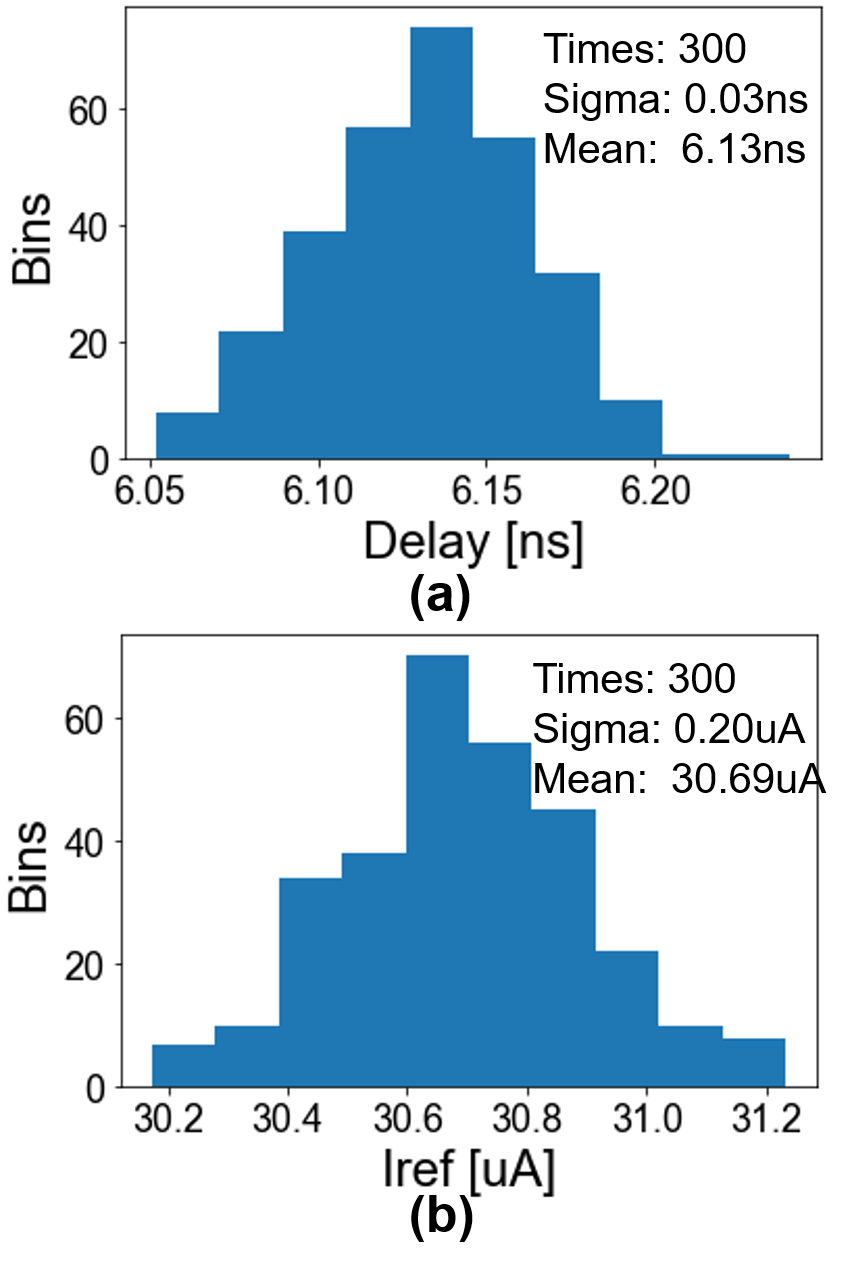
\includegraphics[width=0.35\textwidth]{figs/mc.png}
  \caption{(a) Monte-Carlo simulation results of the CSD delay. (b) Monte-Carlo simulation results of the TBCS $I_{ref}$ under typical conditions.
}
\label{monte}
\end{figure}

% 試作と方針説明
The prototype TBCS was fabricated with 28nm CMOS and the chip photograph is shown in Fig. \ref{chip}. TBCS occupies a very small area of $46um \times 26um$ (0.0012$mm^2$). Unlike the BGR, TBCS does not require bipolar transistors or amplifiers and can be easily designed in advanced CMOS with low supply voltage. Since bipolar transistors and opamps have poor CMOS scaling characteristics, realizing them in scaled CMOS results in a relatively high cost.

In the prototype chip, the TBCS is integrated into the ADC of ref.\cite{yoshioka201728}. Since the prototype does not have an $I_{ref}$ monitoring pin, it was not possible to directly measure the detailed characteristics of the TBCS, and simulation analysis is mainly reported in this paper\footnote{For NDA reasons, all simulation results are reported based on the circuit reimplemented in 65nm CMOS}. On the other hand, we confirmed successful SC and ADC operation over a wide range of environmental variations by measurements, which suggests that TBCS is fully functioning. The TBCS integrated SC circuit and the ADC evaluation results are shown in Fig.\ref{scap} and Fig.\ref{sndr}, respectively. The SC circuit employs two-stage amplification: the opamp biased by TBCS performing the coarse amplification and the successive approximation circuit performs the fine amplification. The ADC achieves a high SNDR (60dB) at a range of -40 to 125$\degC$, and note that such accuracy cannot be obtained if neither the TBCS nor the opamp is not functioning. 

% 電流源としての性能評価
Next, we compare the $I_{ref}$ of BGR current source (BGR ref) as in Fig.\ref{bandgap} and TBCS, respectively. Fig.\ref{iref_pvt_both} shows the simulation results of both current sources under the written PVT variations. The BGR ref with poly-resistors has a large sensitivity to manufacturing variations, and the min-max current value is more than 30uA throughout the variations. The variance is especially large at SSLTLV conditions, where $I_{ref}$ drops by 40\% compared to typical conditions.
Since this corner condition is where the opamp speed is most severe, it will become more challenging to satisfy the target opamp GBW. If $I_{ref}$ will enlarge in such PVT conditions, the design margin can be relaxed and power overhead can be reduced.

In addition, the large $I_{ref}$ increase in the FF condition also poses a problem: the increase in $I_{ref}$ requires to increase the transistor $V_{gs}$ which may narrow down the output range of the opamp. To summarize, to make robust opamp characteristics, it is desirable that $I_{ref}$ increases in the SS condition and decreases in the FF condition.

On the other hand, the simulated TBCS $I_{ref}$ is reported in Fig. \ref{iref_pvt_both}. The input clock frequency is 80MHz, and the TBCS is designed to output 30uA. The main difference between TBCS and BGR ref is the min-max current divergence under PVT. In contrast to BGR, which has a min-max difference of 30uA due to resistance variation, the TBCS reduces the variation width to half (14uA) thanks to the delay-locking feature.

% GBWのシミュレーション結果
The opamp GBW simulation results are reported in Fig.\ref{iref_gbw}, where the opamp was biased with BGR, ideal, and TBCS current sources at different PVT variations, respectively. Identical to the simulation in Fig.\ref{cvar}, we simulate via a simple two-stage differential opamp implemented inside an SC circuit.
As discussed, since the BGR ref reduces its current in the SS condition, the GBW is significantly reduced as well. In the worst corner, the opamp GBW degrades by almost 30\% which can greatly increase the opamp design margin.
On the other hand, TBCS can track PVT with delay-locking and the obtained worst-case opamp GBW is almost the same as that of the ideal current source. Even in the worst corner, the GBW degradation is only 18\%, which is only half of that of BGR ref. Thus, TBCS significantly relaxes the opamp design margin and contributes to reducing the system power consumption.

% monte
Fig.\ref{monte} shows the results of the TBCS Monte Carlo analysis. The overall delay variation is about $\sigma= 30 ps$ in this design, which is small enough compared to the TDC LSB step of 600 ps. As can be seen from the results of Fig.\ref{monte}(b), the effect of mismatch on $I_{ref}$ is also small compared to the current resolution of 1.3uA. %If a more accurate current generation is demanded, a finer TDC LSB will be required and the CSD variation may be reduced.


\section{Conclusions}
Time-Based Current Source (TBCS), a reference current source circuit for SC circuits suitable for scaled CMOS, was proposed. TBCS utilizes the input clock time information and delay-locking. Since the delay is mainly determined by the load capacitors, the generated current is decoupled from resistor values and enables a robust reference current source.  Simulation results showed that the TBCS can half the current variation compared to a bandgap current source under wide PVT variations. When used as the opamp's bias, TBCS achieves the same opamp GBW as an ideal current source through PVT variations. In addition, TBCS is realized mainly with digital circuits and consumed a very small area of 1200$um^2$ when fabricated with 28nm CMOS.

\bibliographystyle{IEEEbib}
\bibliography{main}

\begin{IEEEbiography}
[{
\includegraphics[width=1in,height=1.25in,clip,keepaspectratio]{bio/1.jpg}}]{Kentaro Yoshioka}
received his BS, MS, Ph.D degrees from Keio University, Japan. Currently, he is an Assistant Professor at Keio University. He worked with Toshiba during 2014-2021, developing circuitry for WiFi and LiDAR SoCs. During 2017-2018, he had been a visiting scholar at Stanford University, exploring efficient machine learning hardware and algorithms. 

Currently, Dr. Yoshioka serves as a technical program member of Symp. VLSI circuits conference. He was the recipient of ASP-DAC 2013 Special Feature Award, the A-SSCC 2012 Best Design Award, and 1st place winner of Kaggle 2020 Prostate Cancer Grade Assessment (PANDA) Challenge.
\end{IEEEbiography}

\end{document}
